\documentclass[12pt, letterpaper]{article}
\usepackage{graphicx}
\usepackage[margin=1in]{geometry}
\usepackage{amsmath, amssymb, amsthm, mathrsfs}
\usepackage{fancyhdr}
\usepackage{tikz}
\usepackage{enumerate}
\usepackage{cancel}
\usetikzlibrary{positioning}
\usepackage[utf8]{inputenc}
\usepackage{xcolor}
\usepackage{framed}
\title{HW 1.3}
\author{Your Name}
\date{\today}
\pagestyle{fancy}
\renewcommand{\headrulewidth}{0pt}
\renewcommand{\footrulewidth}{0pt}
\fancyhf{}
\rhead{
    Zack Abdirashid\\
    3/17/26 \\
    MATH 405
}
\rfoot{Page \thepage}
\begin{document}
\paragraph{\underline{2.2} \\ \\} 
\textbf{6.} Show that there can be no Hamilton circuit in the following graph using both edges $(a,f)$ and $(c,h)$.
\begin{center}
    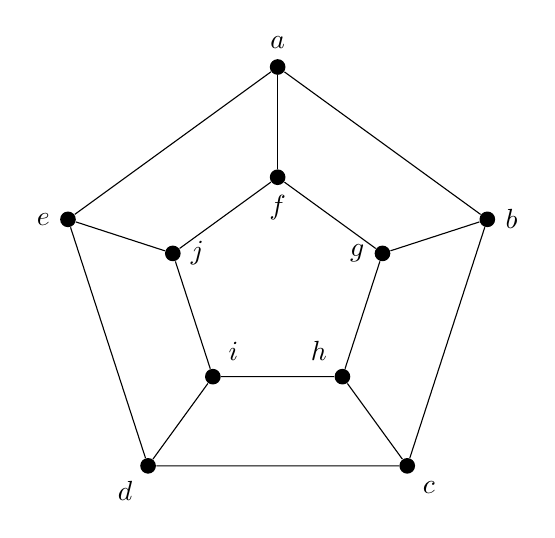
\begin{tikzpicture}[scale=1.4]
        % Outer pentagon vertices
        \node[circle, fill, inner sep=2pt, label=above:$a$]      (a) at (90:2)   {};
        \node[circle, fill, inner sep=2pt, label=right:$b$]      (b) at (18:2)   {};
        \node[circle, fill, inner sep=2pt, label=below right:$c$](c) at (-54:2)  {};
        \node[circle, fill, inner sep=2pt, label=below left:$d$] (d) at (-126:2) {};
        \node[circle, fill, inner sep=2pt, label=left:$e$]       (e) at (162:2)  {};

        % Inner pentagon vertices
        \node[circle, fill, inner sep=2pt, label=below:$f$](f) at (90:1)   {};
        \node[circle, fill, inner sep=2pt, label=left:$g$]      (g) at (18:1)   {};
        \node[circle, fill, inner sep=2pt, label=above left:$h$](h) at (-54:1)  {};
        \node[circle, fill, inner sep=2pt, label=above right:$i$] (i) at (-126:1) {};
        \node[circle, fill, inner sep=2pt, label=right:$j$]       (j) at (162:1)  {};

        % Outer cycle
        \draw (a)--(b)--(c)--(d)--(e)--(a);

        % Spokes
        \draw (a)--(f);
        \draw (b)--(g);
        \draw (c)--(h);
        \draw (d)--(i);
        \draw (e)--(j);

        % Inner pentagram
        \draw (f)--(j)--(i)--(h)--(g)--(f);
    \end{tikzpicture}
\end{center}
- \textbf{Delete} $(a,f)$ and $(c,h)$
\begin{center}
     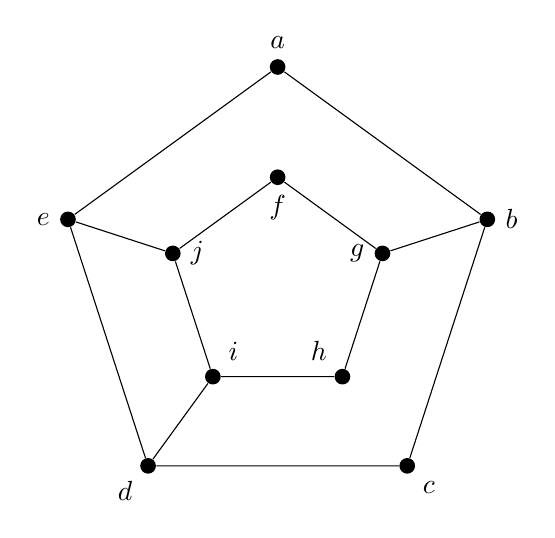
\begin{tikzpicture}[scale=1.4]
        % Outer pentagon vertices
        \node[circle, fill, inner sep=2pt, label=above:$a$]      (a) at (90:2)   {};
        \node[circle, fill, inner sep=2pt, label=right:$b$]      (b) at (18:2)   {};
        \node[circle, fill, inner sep=2pt, label=below right:$c$](c) at (-54:2)  {};
        \node[circle, fill, inner sep=2pt, label=below left:$d$] (d) at (-126:2) {};
        \node[circle, fill, inner sep=2pt, label=left:$e$]       (e) at (162:2)  {};

        % Inner pentagon vertices
        \node[circle, fill, inner sep=2pt, label=below:$f$](f) at (90:1)   {};
        \node[circle, fill, inner sep=2pt, label=left:$g$]      (g) at (18:1)   {};
        \node[circle, fill, inner sep=2pt, label=above left:$h$](h) at (-54:1)  {};
        \node[circle, fill, inner sep=2pt, label=above right:$i$] (i) at (-126:1) {};
        \node[circle, fill, inner sep=2pt, label=right:$j$]       (j) at (162:1)  {};

        % Outer cycle
        \draw (a)--(b)--(c)--(d)--(e)--(a);

        % Spokes
        \draw (b)--(g);
        \draw (d)--(i);
        \draw (e)--(j);

        % Inner pentagram
        \draw (f)--(j)--(i)--(h)--(g)--(f);
    \end{tikzpicture}
\end{center}
- \textbf{Force} $(a,b)$ and $(a,e)$ (deg($a$) = 2) 
\begin{center}
     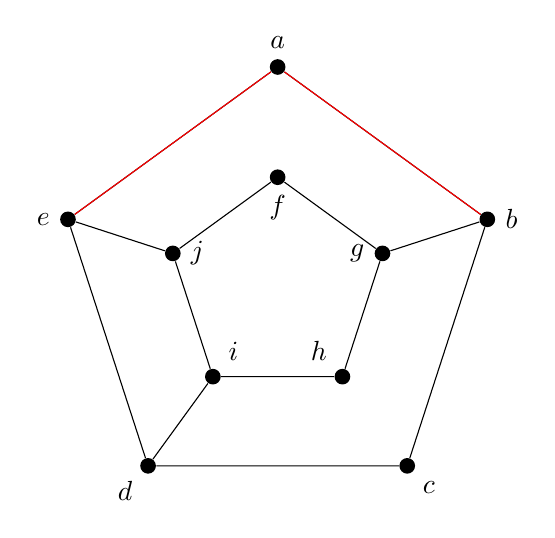
\begin{tikzpicture}[scale=1.4]
        % Outer pentagon vertices
        \node[circle, fill, inner sep=2pt, label=above:$a$]      (a) at (90:2)   {};
        \node[circle, fill, inner sep=2pt, label=right:$b$]      (b) at (18:2)   {};
        \node[circle, fill, inner sep=2pt, label=below right:$c$](c) at (-54:2)  {};
        \node[circle, fill, inner sep=2pt, label=below left:$d$] (d) at (-126:2) {};
        \node[circle, fill, inner sep=2pt, label=left:$e$]       (e) at (162:2)  {};

        % Inner pentagon vertices
        \node[circle, fill, inner sep=2pt, label=below:$f$](f) at (90:1)   {};
        \node[circle, fill, inner sep=2pt, label=left:$g$]      (g) at (18:1)   {};
        \node[circle, fill, inner sep=2pt, label=above left:$h$](h) at (-54:1)  {};
        \node[circle, fill, inner sep=2pt, label=above right:$i$] (i) at (-126:1) {};
        \node[circle, fill, inner sep=2pt, label=right:$j$]       (j) at (162:1)  {};

        % Outer cycle
        \draw (a)--(b)--(c)--(d)--(e)--(a);

        % Spokes
        \draw (b)--(g);
        \draw (d)--(i);
        \draw (e)--(j);
        \draw[red] (a) -- (e);
        \draw[red] (a) -- (b);
        % Inner pentagram
        \draw (f)--(j)--(i)--(h)--(g)--(f);
    \end{tikzpicture} \\
\end{center} \\
- \textbf{Force} $(c,b)$ and $(c,d$) (deg($c$) = 2)
\begin{center}
      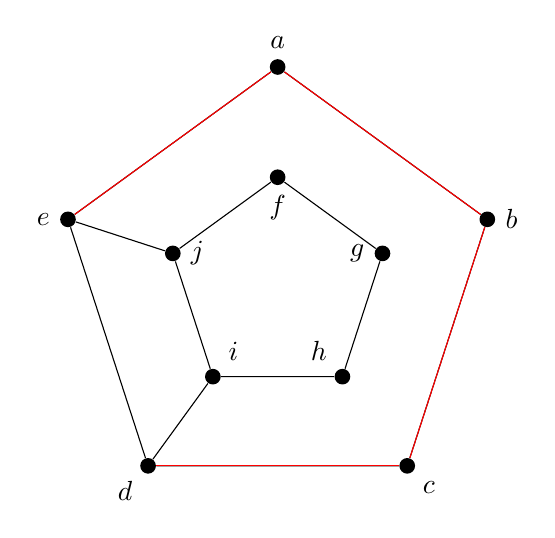
\begin{tikzpicture}[scale=1.4]
        % Outer pentagon vertices
        \node[circle, fill, inner sep=2pt, label=above:$a$]      (a) at (90:2)   {};
        \node[circle, fill, inner sep=2pt, label=right:$b$]      (b) at (18:2)   {};
        \node[circle, fill, inner sep=2pt, label=below right:$c$](c) at (-54:2)  {};
        \node[circle, fill, inner sep=2pt, label=below left:$d$] (d) at (-126:2) {};
        \node[circle, fill, inner sep=2pt, label=left:$e$]       (e) at (162:2)  {};

        % Inner pentagon vertices
        \node[circle, fill, inner sep=2pt, label=below:$f$](f) at (90:1)   {};
        \node[circle, fill, inner sep=2pt, label=left:$g$]      (g) at (18:1)   {};
        \node[circle, fill, inner sep=2pt, label=above left:$h$](h) at (-54:1)  {};
        \node[circle, fill, inner sep=2pt, label=above right:$i$] (i) at (-126:1) {};
        \node[circle, fill, inner sep=2pt, label=right:$j$]       (j) at (162:1)  {};

        % Outer cycle
        \draw (a)--(b)--(c)--(d)--(e)--(a);

        % Spokes
        \draw (d)--(i);
        \draw (e)--(j);
        \draw[red] (a) -- (e);
        \draw[red] (a) -- (b);

        \draw[red] (c) -- (b);
        \draw[red] (c) -- (d);
        % Inner pentagram
        \draw (f)--(j)--(i)--(h)--(g)--(f);
    \end{tikzpicture} \\
    - Delete $(b,g)$ (deg($b$) is 2 after removal) \\
\end{center} 
- \textbf{Force} ($g,h$) and $(g,f)$ (deg($g$) = 2) \\
\begin{center}
      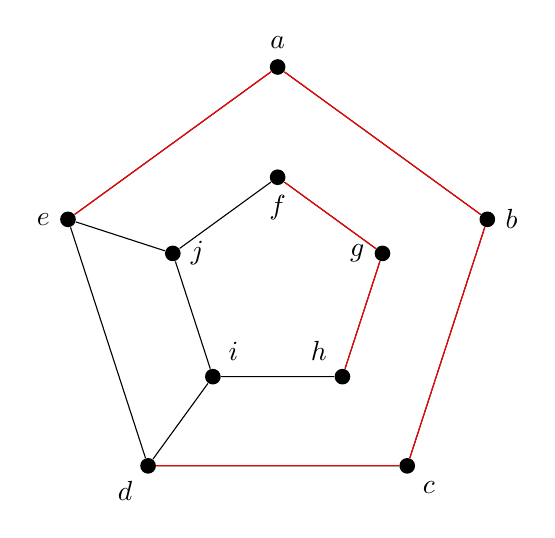
\begin{tikzpicture}[scale=1.4]
        % Outer pentagon vertices
        \node[circle, fill, inner sep=2pt, label=above:$a$]      (a) at (90:2)   {};
        \node[circle, fill, inner sep=2pt, label=right:$b$]      (b) at (18:2)   {};
        \node[circle, fill, inner sep=2pt, label=below right:$c$](c) at (-54:2)  {};
        \node[circle, fill, inner sep=2pt, label=below left:$d$] (d) at (-126:2) {};
        \node[circle, fill, inner sep=2pt, label=left:$e$]       (e) at (162:2)  {};

        % Inner pentagon vertices
        \node[circle, fill, inner sep=2pt, label=below:$f$](f) at (90:1)   {};
        \node[circle, fill, inner sep=2pt, label=left:$g$]      (g) at (18:1)   {};
        \node[circle, fill, inner sep=2pt, label=above left:$h$](h) at (-54:1)  {};
        \node[circle, fill, inner sep=2pt, label=above right:$i$] (i) at (-126:1) {};
        \node[circle, fill, inner sep=2pt, label=right:$j$]       (j) at (162:1)  {};

        % Outer cycle
        \draw (a)--(b)--(c)--(d)--(e)--(a);

        % Spokes
        \draw (d)--(i);
        \draw (e)--(j);
        \draw[red] (a) -- (e);
        \draw[red] (a) -- (b);

        \draw[red] (c) -- (b);
        \draw[red] (c) -- (d);

        % Inner pentagram
        \draw (f)--(j)--(i)--(h)--(g)--(f);
        \draw[red] (g) -- (h);
        \draw[red] (g) -- (f);
    \end{tikzpicture} \\
\end{center} \\
- \textbf{Force} to ($f,j$) and ($h,i$) (deg($f$) = deg($h$) = 2)
\begin{center}
    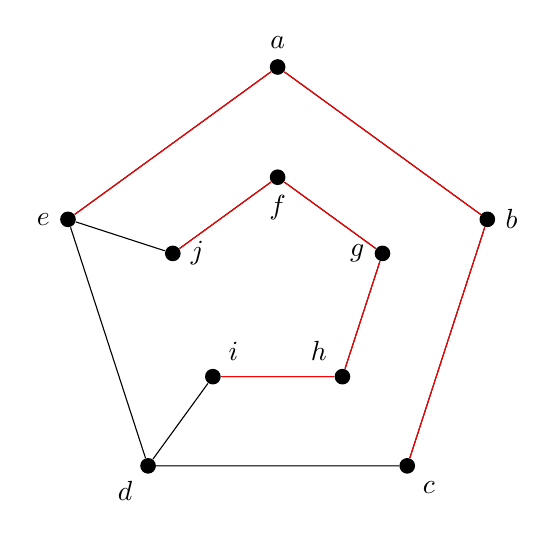
\begin{tikzpicture}[scale=1.4]
        % Outer pentagon vertices
        \node[circle, fill, inner sep=2pt, label=above:$a$]      (a) at (90:2)   {};
        \node[circle, fill, inner sep=2pt, label=right:$b$]      (b) at (18:2)   {};
        \node[circle, fill, inner sep=2pt, label=below right:$c$](c) at (-54:2)  {};
        \node[circle, fill, inner sep=2pt, label=below left:$d$] (d) at (-126:2) {};
        \node[circle, fill, inner sep=2pt, label=left:$e$]       (e) at (162:2)  {};

        % Inner pentagon vertices
        \node[circle, fill, inner sep=2pt, label=below:$f$](f) at (90:1)   {};
        \node[circle, fill, inner sep=2pt, label=left:$g$]      (g) at (18:1)   {};
        \node[circle, fill, inner sep=2pt, label=above left:$h$](h) at (-54:1)  {};
        \node[circle, fill, inner sep=2pt, label=above right:$i$] (i) at (-126:1) {};
        \node[circle, fill, inner sep=2pt, label=right:$j$]       (j) at (162:1)  {};

        % Outer cycle
        \draw (a)--(b)--(c)--(d)--(e)--(a);

        % Spokes
        \draw (d)--(i);
        \draw (e)--(j);
        \draw[red] (a) -- (e);
        \draw[red] (a) -- (b);

        \draw[red] (c) -- (b);
        \draw[red] (c) -- (d);

        % Inner pentagram
        \draw (f)--(j);
        \draw (i)--(h)--(g)--(f);
        \draw[red] (g) -- (h);
        \draw[red] (g) -- (f);

        \draw[red] (f) -- (j);
        \draw[red] (h) -- (i);
    \end{tikzpicture} \\
    - Delete ($j$, $i$) (Creates the sub-circuit $f-g-h-i-j-f$)
\end{center}
\textbf{Force} ($d,i$) and ($e,j$) (deg($i$) = deg($j$) = 2)
    \begin{center}
    \begin{tikzpicture}[scale=1.4]
        % Outer pentagon vertices
        \node[circle, fill, inner sep=2pt, label=above:$a$]      (a) at (90:2)   {};
        \node[circle, fill, inner sep=2pt, label=right:$b$]      (b) at (18:2)   {};
        \node[circle, fill, inner sep=2pt, label=below right:$c$](c) at (-54:2)  {};
        \node[circle, fill, inner sep=2pt, label=below left:$d$] (d) at (-126:2) {};
        \node[circle, fill, inner sep=2pt, label=left:$e$]       (e) at (162:2)  {};

        % Inner pentagon vertices
        \node[circle, fill, inner sep=2pt, label=below:$f$](f) at (90:1)   {};
        \node[circle, fill, inner sep=2pt, label=left:$g$]      (g) at (18:1)   {};
        \node[circle, fill, inner sep=2pt, label=above left:$h$](h) at (-54:1)  {};
        \node[circle, fill, inner sep=2pt, label=above right:$i$] (i) at (-126:1) {};
        \node[circle, fill, inner sep=2pt, label=right:$j$]       (j) at (162:1)  {};

        % Outer cycle
        \draw (a)--(b)--(c)--(d);
        \draw (e)--(a);

        % Spokes
        \draw (d)--(i);
        \draw (e)--(j);
        \draw[red] (a) -- (e);
        \draw[red] (a) -- (b);

        \draw[red] (c) -- (b);
        \draw[red] (c) -- (d);

        % Inner pentagram
        \draw (f)--(j);
        \draw (i)--(h)--(g)--(f);
        \draw[red] (g) -- (h);
        \draw[red] (g) -- (f);

        \draw[red] (f) -- (j);
        \draw[red] (h) -- (i);

        \draw[red] (d) -- (i);
        \draw[red] (e) -- (j);

        \draw[dashed] (a) -- (f);
        \draw[dashed] (c) -- (h)
    \end{tikzpicture} \\
    - Delete ($e$, $d$) (deg($e$) and deg($d$) is 2 after removal) 
\end{center}
\begin{center}
    $\exists$ a H.C: $a-b-c-d-i-h-g-f-j-e-a$. 
\end{center}
\Rightarrow \[
\boxed{
\begin{aligned}
&\text{Cannot use } (a,f) \text{ and } (c,h) \text{ because it would make }
\deg(a), \deg(f), \deg(c) \ \text{and} \deg(h) = 3,\\
&\text{which is impossible for a H.C.}
\end{aligned}
}
\]
\end{center}
\vspace{0.2em}
\textbf{9.} Recall that a graph is \textit{bipartite} if the vertices can be divided into two sets; for convenience call them blue vertices and red vertices, such that every edge connects a blue and a red vertex. \\ \\
\indent \textbf{(a)} Show that if a connected bipartite graph has a Hamilton circuit, then the number of red and blue vertices must be equal. Further, show that if a bipartite graph has an odd number of vertices, then it has no Hamilton circuit.
\begin{proof}
    Suppose $G$ is a connected bipartite graph with a Hamilton circuit. Let $R$ and $B$ be the independent sets of red and blue vertices in $G$. Since $G$ has a Hamilton circuit and every edge connects a red and blue vertex, every vertex in $G$ is not only reached but the H.C alternates between a red and blue vertex. So, it must be that $|R| = |B|$. Suppose $G$ contained an odd \# of vertices. Since $G$ is bipartite, every circuit in $G$ must be of even length. But, a graph of odd vertices would create a circuit of odd length, which is impossible for a bipartite graph. Hence, a Hamilton circuit can not exist in a graph with an odd \# of vertices.
\end{proof}
\indent \textbf{(b)} Show that if a connected bipartite graph has a Hamilton path, then the numbers of reds and blues can differ by at most one.
\begin{proof}
    Let $G$ be a connected bipartite graph that has a Hamilton path $P$. We know that $P$ must reach every vertex in $G$. By contradiction, suppose the \# of red and blue vertices differ by \underline{at least} $2$. Let $R$ be the set of red vertices and $B$ be the set of blue vertices and let $r_{1} \in R$ and $b_{1} \in B$. WLOG let $|B| \geq (|R| + 2)$. \\ 
    \textbf{Case 1}: \ Suppose we start at $r_{1}$ such that
    \begin{align*}
        P = r_{1} - b_{1} - r_{2}-b_{2} - \ldots - r_n - b_n.
    \end{align*}
    But, since $|B| > |R| $, $b_n$ is not the last vertex in $B$. So, vertices
    \begin{align*}
        b_{n+1}, b_{n+2}, \ldots, b_{n+k} \ \text{where $k = |R|$}
    \end{align*}
    will be unreached, contradicting $P$ being a Hamilton path.  \\ 
    \textbf{Case 2}: \ Suppose we start at $b_{1}$ such that
    \begin{align*}
        P = b_{1} - r_{1} - b_{2} - r_{2} - \ldots - b_{n} - r_{n} - b_{n+1}.
    \end{align*}
    The same problem arises in which vertices after $b_{n+1}$ will be unreached, contradicting $P$ being a Hamilton path. Hence, the difference of $|R|$ and $|B|$ must differ by at most $1$ for $G$ to have a Hamilton path.
\end{proof} 
\hspace{0.2em} \\
\indent \textbf{(c)} Use part $(a)$ to show that the following graphs have no Hamilton circuit: \\ \\
    \indent \quad (i) \\
    \indent \quad \begin{center}
    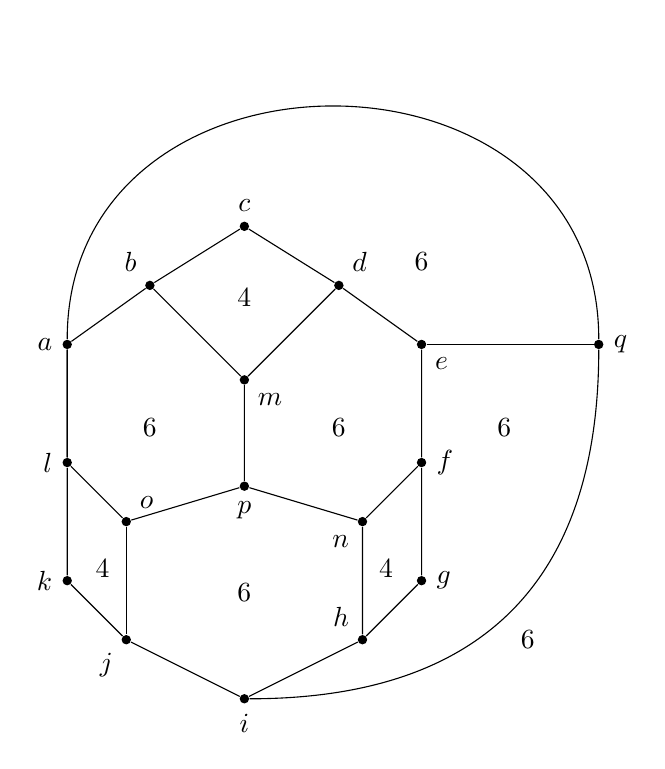
\begin{tikzpicture}[scale=1.5, vertex/.style={circle, fill=black, inner sep=1.2pt}]
        
        % Define coordinates for vertices
        % Central vertices
        \node[vertex, label=above right:$o$] (o) at (-0.5, 0) {};
        \node[vertex, label=below:$p$] (p) at (0.5, 0.3) {};
        \node[vertex, label=below left:$n$] (n) at (1.5, 0) {};
        \node[vertex, label=below right:$m$] (m) at (0.5, 1.2) {};
        
        % Inner ring / Outer hexagon vertices
        \node[vertex, label=left:$l$] (l) at (-1, 0.5) {};
        \node[vertex, label=left:$a$] (a) at (-1, 1.5) {};
        \node[vertex, label=above left:$b$] (b) at (-0.3, 2) {};
        \node[vertex, label=above:$c$] (c) at (0.5, 2.5) {};
        \node[vertex, label=above right:$d$] (d) at (1.3, 2) {};
        \node[vertex, label= below right:$e$] (e) at (2, 1.5) {};
        \node[vertex, label=right:$f$] (f) at (2, 0.5) {};
        \node[vertex, label=right:$g$] (g) at (2, -0.5) {};
        \node[vertex, label=above left:$h$] (h) at (1.5, -1) {};
        \node[vertex, label=below:$i$] (i) at (0.5, -1.5) {};
        \node[vertex, label=below left:$j$] (j) at (-0.5, -1) {};
        \node[vertex, label=left:$k$] (k) at (-1, -0.5) {};
        
        % Far right vertex
        \node[vertex, label=right:$q$] (q) at (3.5, 1.5) {};

        % Draw Edges
        \draw (a) -- (b) -- (c) -- (d) -- (e) -- (f) -- (g) -- (h) -- (i) -- (j) -- (k) -- (l) -- (a);
        \draw (b) -- (m) -- (d);
        \draw (a) -- (l) -- (o) -- (p) -- (m);
        \draw (p) -- (n) -- (f);
        \draw (o) -- (j);
        \draw (n) -- (h);
        \draw (e) -- (q);
        
        % Curved edges
        \draw (a) to [out=90, in=90, looseness=1.5] (q);
        \draw (i) to [out=0, in=270, looseness=1.2] (q);

        % Face Labels (Numbers inside the regions)
        \node at (0.5, 1.9) {4};   % Region b-c-d-m
        \node at (0.5, -0.6) {6}; % Region o-p-n-h-i-j
        \node at (-0.3, 0.8) {6};  % Region a-b-m-p-o-l
        \node at (1.3, 0.8) {6};   % Region m-d-e-f-n-p
        \node at (-0.7, -0.4) {4}; % Region l-o-j-k
        \node at (1.7, -0.4) {4};  % Region n-f-g-h
        \node at (2, 2.2) {6};     % Region a-c-q (upper)
        \node at (2.7, 0.8) {6};   % Region e-q-f-g? (middle right)
        \node at (2.9, -1) {6};  % Region i-q (lower)
    \end{tikzpicture} \\ \\
    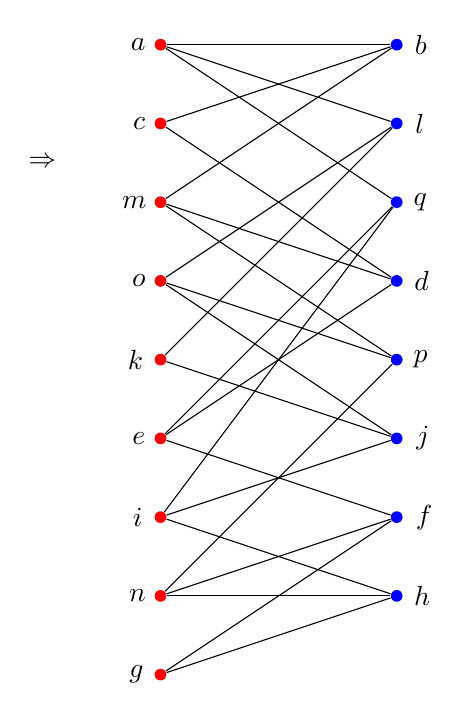
\begin{tikzpicture}[every node/.style={circle,fill,minimum size=1px,inner sep=1.5pt}]
    \node[fill=none, inner sep=0pt] at (-1.5,1.5) {$\Rightarrow$};
    \node[fill=red,label=180:$a$] (a) at (0,3) {};
    \node[fill=red,label=180:$c$] (c) at (0,2) {};
    \node[fill=red,label=180:$m$] (m) at (0,1) {};
    \node[fill=red,label=180:$o$] (o) at (0,0) {};
    \node[fill=red,label=180:$k$] (k) at (0, -1) {};
    \node[fill=red,label=180:$e$] (e) at (0, -2) {};
    \node[fill=red,label=180:$i$] (i) at (0, -3) {};
    \node[fill=red,label=180:$n$] (n) at (0, -4){};
    \node[fill=red,label=180:$g$] (g) at (0, -5) {};
    
    \node[fill=blue,label=0:$b$] (b) at (3,3) {};
    \node[fill=blue,label=0:$l$] (l) at (3,2) {};
    \node[fill=blue,label=0:$q$] (q) at (3,1) {};
    \node[fill=blue,label=0:$d$] (d) at (3,0) {};
    \node[fill=blue,label=0:$p$] (p) at (3, -1) {};
    \node[fill=blue,label=0:$j$] (j) at (3, -2){};
    \node[fill=blue,label=0:$f$] (f) at (3, -3) {};
    \node[fill=blue,label=0:$h$] (h) at (3, -4) {};
    
    \draw (a) -- (b);
    \draw (a) -- (l);
    \draw (a) -- (q);
    
    \draw (c) -- (b);
    \draw (c) -- (d);

    \draw (m) -- (b);
    \draw (m) -- (d);
    \draw (m) -- (p);

    \draw (o) -- (l);
    \draw (o) -- (p);
    \draw (o) -- (j);

    \draw (k) -- (l);
    \draw (k) -- (j);

    \draw (e) -- (q);
    \draw (e) -- (d);
    \draw (e) -- (f);

    \draw (i) -- (q);
    \draw (i) -- (j);
    \draw (i) -- (h);

    \draw (n) -- (p);
    \draw (n) -- (f);
    \draw (n) -- (h);
    
    \draw (g) -- (f);
    \draw (g) -- (h);
\end{tikzpicture} \\
\Rightarrow \ \text{$G$ is bipartite!}
\end{center} 
\begin{align*}
    \boxed{\text{But G has 17 vertices which is odd. So, no Hamilton circuit exists.}}
\end{align*} 
\hspace{0.2em}
\indent \quad (ii)
\indent \quad \begin{center}
    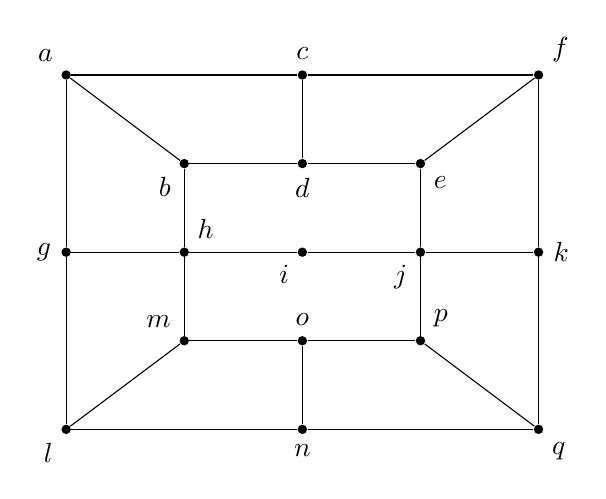
\begin{tikzpicture}[scale=1.5, vertex/.style={circle, fill=black, inner sep=1.2pt}]
        
        % Define coordinates for the 3x3 grid of vertices
        % Outer Rectangle
        \node[vertex, label=above left:$a$] (a) at (-2, 1.5) {};
        \node[vertex, label=above:$c$] (c) at (0, 1.5) {};
        \node[vertex, label=above right:$f$] (f) at (2, 1.5) {};
        
        \node[vertex, label=left:$g$] (g) at (-2, 0) {};
        \node[vertex, label=below left:$i$] (i) at (0, 0) {}; % Label slightly offset
        \node[vertex, label=right:$k$] (k) at (2, 0) {};
        
        \node[vertex, label=below left:$l$] (l) at (-2, -1.5) {};
        \node[vertex, label=below:$n$] (n) at (0, -1.5) {};
        \node[vertex, label=below right:$q$] (q) at (2, -1.5) {};

        % Inner Rectangle
        \node[vertex, label=below left:$b$] (b) at (-1, 0.75) {};
        \node[vertex, label=below:$d$] (d) at (0, 0.75) {};
        \node[vertex, label=below right:$e$] (e) at (1, 0.75) {};
        
        \node[vertex, label=above right:$h$] (h) at (-1, 0) {};
        \node[vertex, label=below left:$j$] (j) at (1, 0) {};
        
        \node[vertex, label=above left:$m$] (m) at (-1, -0.75) {};
        \node[vertex, label=above:$o$] (o) at (0, -0.75) {};
        \node[vertex, label=above right:$p$] (p) at (1, -0.75) {};

        % Draw Horizontal Edges
        \draw (a) -- (c) -- (f);
        \draw (g) -- (h) -- (i) -- (j) -- (k);
        \draw (l) -- (n) -- (q);
        \draw (b) -- (d) -- (e);
        \draw (m) -- (o) -- (p);

        % Draw Vertical Edges
        \draw (a) -- (g) -- (l);
        \draw (c) -- (d);
        \draw (o) -- (n);
        \draw (f) -- (k) -- (q);
        \draw (b) -- (h) -- (m);
        \draw (e) -- (j) -- (p);

        % Draw Diagonal Edges
        \draw (a) -- (b);
        \draw (f) -- (e);
        \draw (l) -- (m);
        \draw (q) -- (p);

    \end{tikzpicture} \\ 
    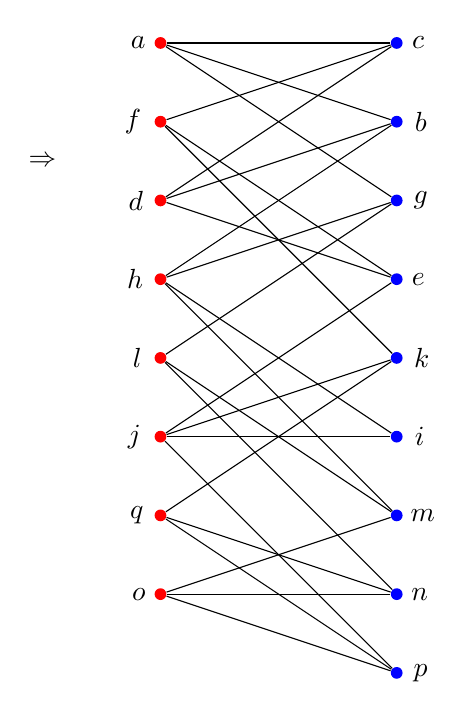
\begin{tikzpicture}[every node/.style={circle,fill,minimum size=1px,inner sep=1.5pt}]
    \node[fill=none, inner sep=0pt] at (-1.5,1.5) {$\Rightarrow$};
    \node[fill=red,label=180:$a$] (a) at (0,3) {};
    \node[fill=red,label=180:$f$] (f) at (0,2) {};
    \node[fill=red,label=180:$d$] (d) at (0,1) {};
    \node[fill=red,label=180:$h$] (h) at (0,0) {};
    \node[fill=red,label=180:$l$] (l) at (0, -1) {};
    \node[fill=red,label=180:$j$] (j) at (0, -2) {};
    \node[fill=red,label=180:$q$] (q) at (0, -3) {};
    \node[fill=red,label=180:$o$] (o) at (0, -4){};
    
    \node[fill=blue,label=0:$c$] (c) at (3,3) {};
    \node[fill=blue,label=0:$b$] (b) at (3,2) {};
    \node[fill=blue,label=0:$g$] (g) at (3,1) {};
    \node[fill=blue,label=0:$e$] (e) at (3,0) {};
    \node[fill=blue,label=0:$k$] (k) at (3, -1) {};
    \node[fill=blue,label=0:$i$] (i) at (3, -2){};
    \node[fill=blue,label=0:$m$] (m) at (3, -3) {};
    \node[fill=blue,label=0:$n$] (n) at (3, -4) {};
    \node[fill=blue,label=0:$p$] (p) at (3, -5) {};
    
    \draw (a) -- (c);
    \draw (a) -- (b);
    \draw (a) -- (g);
    
    \draw (f) -- (c);
    \draw (f) -- (e);
    \draw (f) -- (k);

    \draw (d) -- (c);
    \draw (d) -- (b);
    \draw (d) -- (e);

    \draw (h) -- (b);
    \draw (h) -- (g);
    \draw (h) -- (i);
    \draw(h) -- (m);

    \draw (l) -- (g);
    \draw (l) -- (m);
    \draw (l) -- (n);

    \draw (j) -- (e);
    \draw (j) -- (k);
    \draw (j) -- (i);
    \draw (j) -- (p);

    \draw (q) -- (k);
    \draw (q) -- (n);
    \draw (q) -- (p);

    \draw (o) -- (m);
    \draw (o) -- (n);
    \draw (o) -- (p);
\end{tikzpicture} \\
\Rightarrow \ \text{$G$ is bipartite!}
\end{center}
\begin{align*}
    \boxed{\text{But $G$ has 17 vertices which is odd. So, no H. C exists.}}
\end{align*}
\hspace{0.2em}
\indent \quad (iii)
\indent \quad \begin{center}
    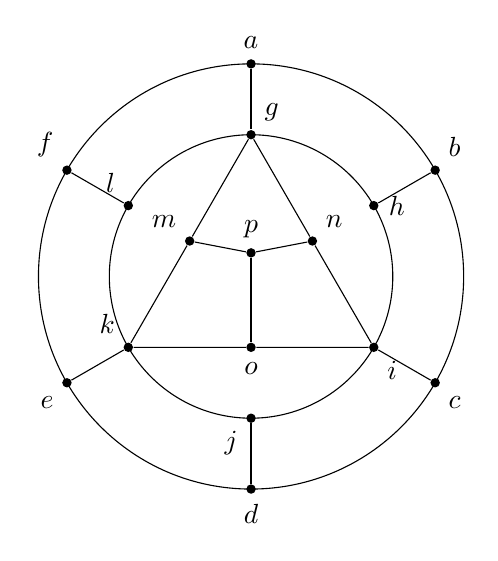
\begin{tikzpicture}[scale=1.5, vertex/.style={circle, fill=black, inner sep=1.2pt}]

        % Outer Circle Vertices (Radius 1.8)
        \node[vertex, label=above:$a$] (a) at (90:1.8) {};
        \node[vertex, label=above right:$b$] (b) at (30:1.8) {};
        \node[vertex, label=below right:$c$] (c) at (330:1.8) {};
        \node[vertex, label=below:$d$] (d) at (270:1.8) {};
        \node[vertex, label=below left:$e$] (e) at (210:1.8) {};
        \node[vertex, label=above left:$f$] (f) at (150:1.8) {};

        % Inner Circle Vertices (Radius 1.2)
        \node[vertex, label=above right:$g$] (g) at (90:1.2) {};
        \node[vertex, label=right:$h$] (h) at (30:1.2) {};
        \node[vertex, label=below right:$i$] (i) at (330:1.2) {};
        \node[vertex, label=below left:$j$] (j) at (270:1.2) {};
        \node[vertex, label=above left:$k$] (k) at (210:1.2) {};
        \node[vertex, label=above left:$l$] (l) at (150:1.2) {};

        % Triangle/Inner Structure Vertices
        \node[vertex, label=above left:$m$] (m) at (150:0.6) {};
        \node[vertex, label=above right:$n$] (n) at (30:0.6) {};
        \node[vertex, label=below:$o$] (o) at (270:0.6) {};
        \node[vertex, label=above:$p$] (p) at (0, 0.2) {}; % Slightly above center

        % Draw Circles
        \draw (0,0) circle (1.8);
        \draw (0,0) circle (1.2);

        % Draw Radial Spokes
        \draw (a) -- (g);
        \draw (b) -- (h);
        \draw (c) -- (i);
        \draw (d) -- (j);
        \draw (e) -- (k);
        \draw (f) -- (l);

        % Draw Internal Triangle and Central connections
        \draw (g) -- (m) -- (k);
        \draw (k) -- (o) -- (i);
        \draw (i) -- (n) -- (g);
        
        % Connections to center point p
        \draw (m) -- (p);
        \draw (n) -- (p);
        \draw (o) -- (p);

    \end{tikzpicture} \\
        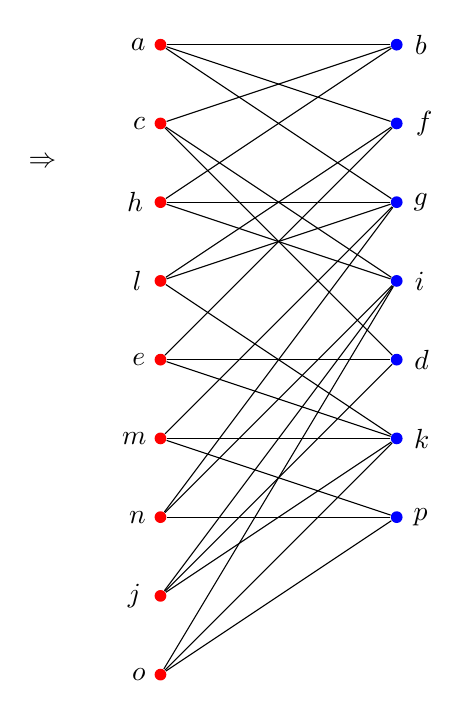
\begin{tikzpicture}[every node/.style={circle,fill,minimum size=1px,inner sep=1.5pt}]
    \node[fill=none, inner sep=0pt] at (-1.5,1.5) {$\Rightarrow$};
    \node[fill=red, label=180:$a$] (a) at (0,3) {};
    \node[fill=red,label=180:$c$] (c) at (0,2) {};
    \node[fill=red,label=180:$h$] (h) at (0,1) {};
    \node[fill=red,label=180:$l$] (l) at (0,0) {};
    \node[fill=red,label=180:$e$] (e) at (0, -1) {};
    \node[fill=red,label=180:$m$] (m) at (0, -2) {};
    \node[fill=red,label=180:$n$] (n) at (0, -3) {};
    \node[fill=red,label=180:$j$] (j) at (0, -4){};
    \node[fill=red,label=180:$o$] (o) at (0, -5){};
    
    \node[fill=blue,label=0:$b$] (b) at (3,3) {};
    \node[fill=blue,label=0:$f$] (f) at (3,2) {};
    \node[fill=blue,label=0:$g$] (g) at (3,1) {};
    \node[fill=blue,label=0:$i$] (i) at (3,0) {};
    \node[fill=blue,label=0:$d$] (d) at (3, -1) {};
    \node[fill=blue,label=0:$k$] (k) at (3, -2){};
    \node[fill=blue,label=0:$p$] (p) at (3, -3) {};
    
    \draw (b) -- (a);
    \draw (b) -- (c);
    \draw (b) -- (h);

    \draw (f) -- (a);
    \draw (f) -- (l); 
    \draw (f) -- (e);

    \draw (g) -- (a);
    \draw (g) -- (h);
    \draw (g) -- (l);
    \draw (g) -- (m);
    \draw (g) -- (n);

    \draw (i) -- (c);
    \draw (i) -- (h);
    \draw (i) -- (n);
    \draw (i) -- (o);
    \draw (i) -- (j);

    \draw (d) -- (j);
    \draw (d) -- (e);
    \draw (d) -- (c);

    \draw (k) -- (e);
    \draw (k) -- (l);
    \draw (k) -- (j);
    \draw (k) -- (m);
    \draw (k) -- (o);

    \draw (p) -- (m);
    \draw (p) -- (n);
    \draw (p) -- (o);
\end{tikzpicture} \\
\Rightarrow \ \text{$G$ is bipartite!}
\end{center} 
\begin{align*}
    \boxed{\text{But $|R| = 9 \neq |B| = 7$. So, no H.C exists.}}
\end{align*}
\vspace{0.2em}
\textbf{7(a).} Prove that the following graph has no Hamilton circuit. (*Use Theorem 3)
\begin{center}
    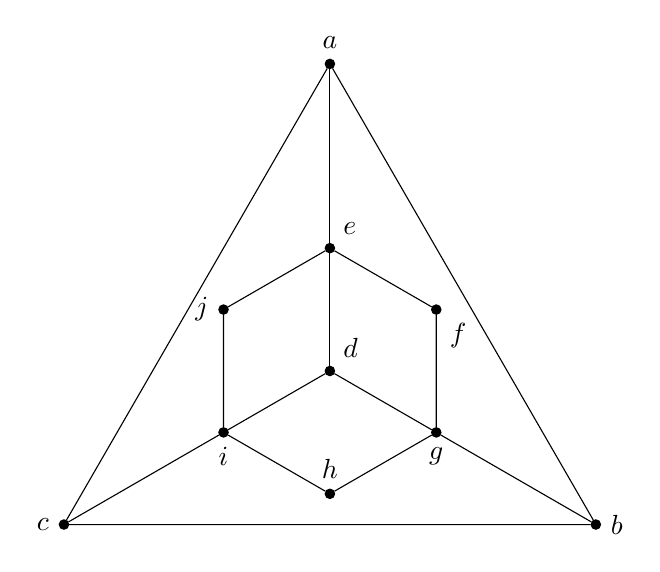
\begin{tikzpicture}[scale=1.3, auto, swap]
    % Define the vertices
    % Outer Triangle (a, b, c)
    \node[draw, circle, fill=black, inner sep=1.2pt, label=above:{$a$}] (a) at (90:3) {};
    \node[draw, circle, fill=black, inner sep=1.2pt, label=right:{$b$}] (b) at (-30:3) {};
    \node[draw, circle, fill=black, inner sep=1.2pt, label=left:{$c$}] (c) at (210:3) {};

    % Inner Hub (d)
    \node[draw, circle, fill=black, inner sep=1.2pt, label=above right:{$d$}] (d) at (0,0) {};

    % Inner ring vertices (e, f, g, h, i, j)
    \node[draw, circle, fill=black, inner sep=1.2pt, label=above right:{$e$}] (e) at (90:1.2) {};
    \node[draw, circle, fill=black, inner sep=1.2pt, label=below right:{$f$}] (f) at (30:1.2) {};
    \node[draw, circle, fill=black, inner sep=1.2pt, label=below:{$g$}] (g) at (-30:1.2) {};
    \node[draw, circle, fill=black, inner sep=1.2pt, label=above:{$h$}] (h) at (-90:1.2) {};
    \node[draw, circle, fill=black, inner sep=1.2pt, label=below :{$i$}] (i) at (210:1.2) {};
    \node[draw, circle, fill=black, inner sep=1.2pt, label=left:{$j$}] (j) at (150:1.2) {};

    % Draw the Edges
    % Outer Triangle
    \draw (a) -- (b) -- (c) -- (a);

    % Connections from Outer to Inner
    \draw (a) -- (e);
    \draw (b) -- (g);
    \draw (c) -- (i);

    % The Central Hub Edges
    \draw (d) -- (e);
    \draw (d) -- (g);
    \draw (d) -- (i);

    % The Hexagon-like ring
    \draw (e) -- (f) -- (g);
    \draw (g) -- (h) -- (i);
    \draw (i) -- (j) -- (e);

\end{tikzpicture} \\
- Is this graph $G$ planar? yes \\
\end{center}
\begin{center}
    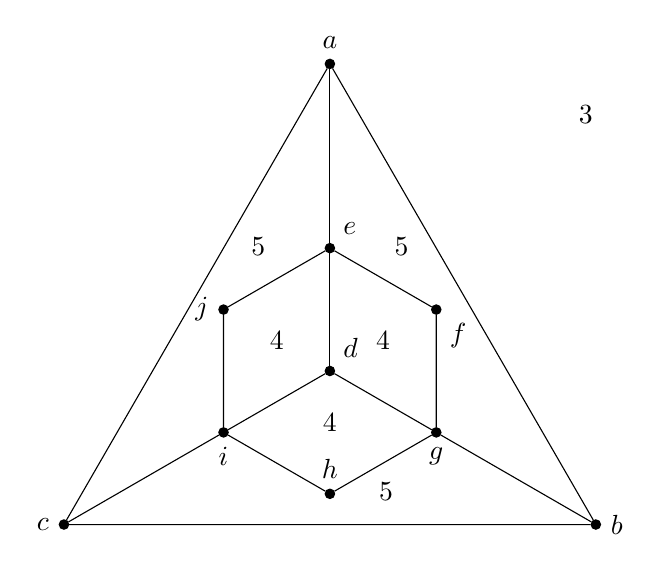
\begin{tikzpicture}[scale=1.3, auto, swap]
    % Define the vertices
    % Outer Triangle (a, b, c)
    \node[draw, circle, fill=black, inner sep=1.2pt, label=above:{$a$}] (a) at (90:3) {};
    \node[draw, circle, fill=black, inner sep=1.2pt, label=right:{$b$}] (b) at (-30:3) {};
    \node[draw, circle, fill=black, inner sep=1.2pt, label=left:{$c$}] (c) at (210:3) {};

    % Inner Hub (d)
    \node[draw, circle, fill=black, inner sep=1.2pt, label=above right:{$d$}] (d) at (0,0) {};

    % Inner ring vertices (e, f, g, h, i, j)
    \node[draw, circle, fill=black, inner sep=1.2pt, label=above right:{$e$}] (e) at (90:1.2) {};
    \node[draw, circle, fill=black, inner sep=1.2pt, label=below right:{$f$}] (f) at (30:1.2) {};
    \node[draw, circle, fill=black, inner sep=1.2pt, label=below:{$g$}] (g) at (-30:1.2) {};
    \node[draw, circle, fill=black, inner sep=1.2pt, label=above:{$h$}] (h) at (-90:1.2) {};
    \node[draw, circle, fill=black, inner sep=1.2pt, label=below :{$i$}] (i) at (210:1.2) {};
    \node[draw, circle, fill=black, inner sep=1.2pt, label=left:{$j$}] (j) at (150:1.2) {};

    % Draw the Edges
    % Outer Triangle
    \draw (a) -- (b) -- (c) -- (a);

    % Connections from Outer to Inner
    \draw (a) -- (e);
    \draw (b) -- (g);
    \draw (c) -- (i);

    % The Central Hub Edges
    \draw (d) -- (e);
    \draw (d) -- (g);
    \draw (d) -- (i);

    % The Hexagon-like ring
    \draw (e) -- (f) -- (g);
    \draw (g) -- (h) -- (i);
    \draw (i) -- (j) -- (e);

    % --- Degree Labels ---
    
    % Degree 4: Inside the three central regions
    \node at (30:0.6) {4};   % Inside (e, f, g, d)
    \node at (270:0.5) {4};  % Inside (d, g, h, i)
    \node at (150:0.6) {4};  % Inside (j, e, d, i)

    % Degree 5: Inside the three outer boundary regions
    \node at (120:1.4) {5};  % Inside (a, c, i, j, e)
    \node at (295:1.3) {5};  % Inside (c, i, h, g, b)
    \node at (60:1.4) {5};   % Inside (b, g, f, e, a)

    % Degree 3: The infinite outer region (placed just outside the boundary)
    \node at (2.5, 2.5) {3}; 

\end{tikzpicture} \\
- Does this graph have a H.C?
\end{center}
\begin{align*}
    \Rightarrow i = 3 \ &\xrightarrow[\text{1 region}]{} \ r_3 + r'_{3} = 1 \\
    \Rightarrow i = 4 \ &\xrightarrow[\text{3 regions}]{} \ r_4 + r_4' = 3 \\
    \Rightarrow i = 5 \ &\xrightarrow[\text{3 regions}]{} \ r_5 + r_5' = 3
\end{align*}
\begin{align*}
    * \ \sum _{i} \ (i-2) (r_i - r_i') = 0
\end{align*}
\begin{align*}
    &\Rightarrow (3-2)(r_3 -r_3') + (4-2)(r_4 - r_4') + (5-2)(r_5 - r_5') = 0 \\  \\
    &\Rightarrow (r_3 - r_3') + 2(r_4 - r_4') + 3(r_5 - r_5')= 0 \\ \\
    &\Rightarrow \pm \{1\} \ \pm \ 2\{1, 3\} \ \pm \ 3\{1, 3\} = 0  \\ \\
    &\Rightarrow \pm \{1\} \ \pm \ \{2, 6\} \ \pm \ \{3, 9\} = 0 \\ \\
    &\Rightarrow \text{inconclusive due to the possible solution $1 + 2 - 3 = 0$}.
\end{align*}
- \textbf{Force} ($j,i$) and ($j,e$) (deg($j$) = 2)
\begin{center}
    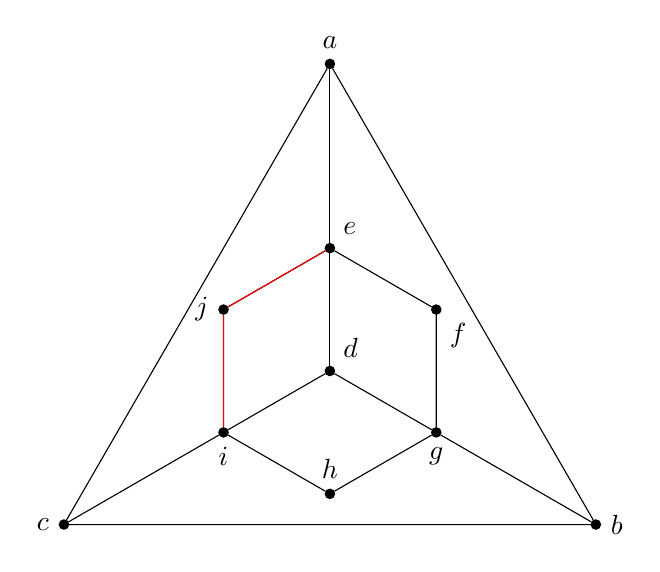
\begin{tikzpicture}[scale=1.3, auto, swap]
    % Define the vertices
    % Outer Triangle (a, b, c)
    \node[draw, circle, fill=black, inner sep=1.2pt, label=above:{$a$}] (a) at (90:3) {};
    \node[draw, circle, fill=black, inner sep=1.2pt, label=right:{$b$}] (b) at (-30:3) {};
    \node[draw, circle, fill=black, inner sep=1.2pt, label=left:{$c$}] (c) at (210:3) {};

    % Inner Hub (d)
    \node[draw, circle, fill=black, inner sep=1.2pt, label=above right:{$d$}] (d) at (0,0) {};

    % Inner ring vertices (e, f, g, h, i, j)
    \node[draw, circle, fill=black, inner sep=1.2pt, label=above right:{$e$}] (e) at (90:1.2) {};
    \node[draw, circle, fill=black, inner sep=1.2pt, label=below right:{$f$}] (f) at (30:1.2) {};
    \node[draw, circle, fill=black, inner sep=1.2pt, label=below:{$g$}] (g) at (-30:1.2) {};
    \node[draw, circle, fill=black, inner sep=1.2pt, label=above:{$h$}] (h) at (-90:1.2) {};
    \node[draw, circle, fill=black, inner sep=1.2pt, label=below :{$i$}] (i) at (210:1.2) {};
    \node[draw, circle, fill=black, inner sep=1.2pt, label=left:{$j$}] (j) at (150:1.2) {};

    % Draw the Edges
    % Outer Triangle
    \draw (a) -- (b) -- (c) -- (a);

    % Connections from Outer to Inner
    \draw (a) -- (e);
    \draw (b) -- (g);
    \draw (c) -- (i);

    % The Central Hub Edges
    \draw (d) -- (e);
    \draw (d) -- (g);
    \draw (d) -- (i);

    % The Hexagon-like ring
    \draw (e) -- (f) -- (g);
    \draw (g) -- (h) -- (i);
    \draw (i) -- (j) -- (e);

    \draw[red] (j) -- (i);
    \draw[red] (j) -- (e);
\end{tikzpicture} \\
\end{center}
- \textbf{Force} ($f,e$) and ($f, g$) (deg($f$) = 2)
\begin{center}
    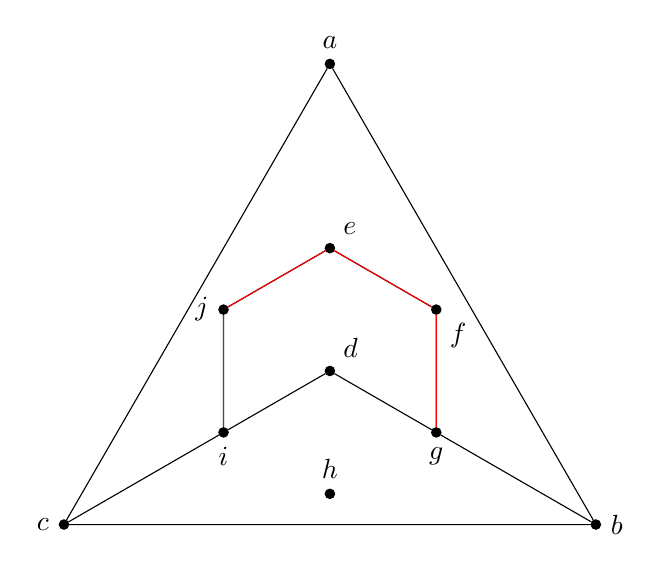
\begin{tikzpicture}[scale=1.3, auto, swap]
    % Define the vertices
    % Outer Triangle (a, b, c)
    \node[draw, circle, fill=black, inner sep=1.2pt, label=above:{$a$}] (a) at (90:3) {};
    \node[draw, circle, fill=black, inner sep=1.2pt, label=right:{$b$}] (b) at (-30:3) {};
    \node[draw, circle, fill=black, inner sep=1.2pt, label=left:{$c$}] (c) at (210:3) {};

    % Inner Hub (d)
    \node[draw, circle, fill=black, inner sep=1.2pt, label=above right:{$d$}] (d) at (0,0) {};

    % Inner ring vertices (e, f, g, h, i, j)
    \node[draw, circle, fill=black, inner sep=1.2pt, label=above right:{$e$}] (e) at (90:1.2) {};
    \node[draw, circle, fill=black, inner sep=1.2pt, label=below right:{$f$}] (f) at (30:1.2) {};
    \node[draw, circle, fill=black, inner sep=1.2pt, label=below:{$g$}] (g) at (-30:1.2) {};
    \node[draw, circle, fill=black, inner sep=1.2pt, label=above:{$h$}] (h) at (-90:1.2) {};
    \node[draw, circle, fill=black, inner sep=1.2pt, label=below :{$i$}] (i) at (210:1.2) {};
    \node[draw, circle, fill=black, inner sep=1.2pt, label=left:{$j$}] (j) at (150:1.2) {};

    % Draw the Edges
    % Outer Triangle
    \draw (a) -- (b) -- (c) -- (a);

    % Connections from Outer to Inner
    \draw (b) -- (g);
    \draw (c) -- (i);

    % The Central Hub Edges
    \draw (d) -- (g);
    \draw (d) -- (i);

    % The Hexagon-like ring
    \draw (e) -- (f) -- (g);
    \draw (i) -- (j) -- (e);

    \draw[red] (j) -- (i);
    \draw[red] (j) -- (e);

    \draw[red] (f) -- (e);
    \draw[red] (f) -- (g);
\end{tikzpicture} \\
- Delete ($e,d$) and ($e,a$) (deg($e$) is 2 after removal) \\
- Delete ($h,g$) and ($h,i$) because of the sub-circuit $e-f-g-h-i-j-e$.
\end{center} \\
\text{Cannot be done because preventing a sub-circuit causes deg($h$) = 0,\
which is impossible in a H.C.}. 
\[
\boxed{
\begin{aligned}
&\text{Exhausted all choices $\therefore$ no H.C exists}
\end{aligned}
}
\]
\end{document}